%%%%%%%%%%%%%%%%%%%%%%%%%%%%%%%%%%%%%%%%%%%%%%%%%%%%%%%%%%%%%%%%%%%%%%%%%%%%%%%%
%2345678901234567890123456789012345678901234567890123456789012345678901234567890
%        1         2         3         4         5         6         7         8

\documentclass[letterpaper, 10 pt, conference]{ieeeconf}  % Comment this line out if you need a4paper

%\documentclass[a4paper, 10pt, conference]{ieeeconf}      % Use this line for a4 paper

\IEEEoverridecommandlockouts                              % This command is only needed if 
                                                          % you want to use the \thanks command

\overrideIEEEmargins                                      % Needed to meet printer requirements.

% See the \addtolength command later in the file to balance the column lengths
% on the last page of the document

% The following packages can be found on http:\\www.ctan.org
%\usepackage{graphics} % for pdf, bitmapped graphics files
%\usepackage{epsfig} % for postscript graphics files
%\usepackage{mathptmx} % assumes new font selection scheme installed
%\usepackage{times} % assumes new font selection scheme installed

%%%%%%%%%% my includes %%%

\usepackage{url}      % needed for ieeetran bib style
\usepackage{graphicx}
\graphicspath{{./03_graphics/}}

% possible subfigure packages
%\usepackage{subfigure}
%\usepackage[caption=false,font=footnotesize]{subfig}

\usepackage[colorinlistoftodos, german]{todonotes} % Option 'disable' entfernt alle ToDos

\usepackage[utf8]{inputenc}

\usepackage[font=footnotesize]{caption}
\usepackage[font=footnotesize]{subcaption}
\newtheorem{thm}{Theorem}[section]
\newtheorem{defn}[thm]{Definition}


\usepackage{hyperref}

%% format tabular cells
\usepackage{booktabs}
\usepackage{tabularx}
\usepackage{makecell}
\renewcommand\theadalign{bc}
\renewcommand\theadfont{\bfseries}
\renewcommand\theadgape{\Gape[4pt]}
\renewcommand\cellgape{\Gape[4pt]}

%\usepackage[style=plain,citestyle=numeric,bibstyle=numeric,sorting=none,url=false,doi=false,isbn=false]{biblatex}

%%%%%%%%%%%%%%%%%%%%%%%%%%


\title{\LARGE \bf
Deep Reinforcement Learning with Continuous Control in CARLA
}

\author{Moritz Zanger$^{1}$ Florian Rottach$^{1}$ Izel Kilinc$^{1}$ % <-this % stops a space
\thanks{$^{1}$The authors are with FZI Research Center for Information Technology, Haid-und-Neu-Str. 10-14, 76131 Karlsruhe, Germany
%        {\tt\small \{kuhnt, zoellner\}@fzi.de}}%
        {\tt\small \{, uzdnz\}@student.kit.edu}}%
}        
        
\begin{document}



\maketitle
\thispagestyle{empty}
\pagestyle{empty}


%%%%%%%%%%%%%%%%%%%%%%%%%%%%%%%%%%%%%%%%%%%%%%%%%%%%%%%%%%%%%%%%%%%%%%%%%%%%%%%%
\begin{abstract}

%This electronic document is a ÒliveÓ template. The various components of your paper [title, text, heads, etc.] are already defined on the style sheet, as illustrated by the portions given in this document.

Style:
\begin{itemize}
	\item Written last
	\item 100-250 words
	\item Past tense
\end{itemize}

Content:
\begin{itemize}
	\item Condensed version of entire article
\end{itemize}

\end{abstract}


%%%%%%%%%%%%%%%%%%%%%%%%%%%%%%%%%%%%%%%%%%%%%%%%%%%%%%%%%%%%%%%%%%%%%%%%%%%%%%%%
\section{Introduction}

%This template provides authors with most of the formatting specifications needed for preparing electronic versions of their papers. All standard paper components have been specified for three reasons: (1) ease of use when formatting individual papers, (2) automatic compliance to electronic requirements that facilitate the concurrent or later production of electronic products, and (3) conformity of style throughout a conference proceedings. Margins, column widths, line spacing, and type styles are built-in; examples of the type styles are provided throughout this document and are identified in italic type, within parentheses, following the example. Some components, such as multi-leveled equations, graphics, and tables are not prescribed, although the various table text styles are provided. The formatter will need to create these components, incorporating the applicable criteria that follow.

%Example Citation: \cite{Barth2008}.

The task of teaching vehicles how to drive autonomously in urban scenarios is a challenging and complex one to solve. Not only is there the problem of finding the adequate response to a given situation but also the challenge of taking into account the surrounding factors that have an influence on the state that a vehicle is in and its possible actions. To date, most approaches focus on the manual design of behavioral policies, such as defining a driving policy through the use of annotated maps. While these solutions might work in situations which are documented by the provided mapping infrastructure, they are often difficult to generalize or scale, as they do not necessarily enable the comprehension of any given local scene. In order to make autonomous driving truly feasible in a real-world scenario it would be better to develop systems which are able to find their way without having to rely on an explicit set of rules. One possible solution to this task is provided by reinforcement learning methods. Here, the agent, i.e. the vehicle, actively searches for the optimal driving policy whilst trying to maximize a numerical reward signal. As opposed to imitation learning techniques, which have been popular in finding driving policies (1), reinforment learning algorithms enable a car to exceed human abilities, if applied correctly. In recent years, deep reinforcement learning methods have proven to be succesful in solving complex tasks such as playing GO (2) or Atari (3) and there have been efforts in tackling various problems in the field of autonomous driving, including continous control tasks (4).

However, two major drawbacks of reinforcement learning methods are their heavy depency on adequate input state representations (5) and, as with other machine learning techniques, their need of a sufficient amount of accurate sample data to train on. In order to be able to train safely on an adequate amount of data, one approach is the use of data from other domains. For this purpose, the urban driving simulator CARLA has been developed, which is used as a simulation environment for this project.

In previous projects, CARLA has been used to learn policies that allow agents to navigate through complex urban environments via imitation learning methods (15)(12). In this paper, it serves as an environment to solve a continuous control task vie deep reinforcement learning. Several state-of-the-art reinforcement learning algorithms are implemented and compared, with regard to their performance considering driving tasks of increasing complexity. Additionally, reward functions for the respective problems are tested and different input represantations are designed and evaluated.

%\subsection{Problem specification}
%\subsection{Why RL? What is our goal/motivation?}

\section{Related Work}

%1. Reinforcement learning tasks have been tackled successfully in the past
%	- discrete control tasks
%	- human performance could be "overcome"
%2. Continuous control is quite a new field
%	- Need different algorithms
%	- Adjustments and new developments have been made
%3. DDPG
%4. A3C
%5. PPO
%6. Autoencoder/DDPG
%7. Birds eye view
%8. CarRacing/TORCS
%9. We extend this to CARLA
%	- Has been done with imitation learning achieving good results
Various reinforcement learning tasks have been tackled successfully in the past, leading to notable advances in learning policies for simulated and real-world robotic control problems (Levine and Koltun, de Bruin et al.) or solving complex game structures (9). The resulting deep reinforcement learning methods have recently been developed so far as to achieving similar results or beating human experts in some of these tasks (2)(8). In their paper, Silver et al. (2) introduce a new approach of teaching an agent the game of GO by combining Monte Carlo simulation with value and policy networks to evaluate board positions and choose new moves. In autonomous driving, Wolf et al. have achieved notable results using a Deep Q Network to evaluate possible steering actions from an action space of five predetermined steering options (10). 

However, many tasks that could be solved with reinforcement learning approaches have continuous action spaces, to which approaches such as the DQN cannot be directly applied in a feasible manner (4). Therefore, algorithms that can handle these high-dimensional action spaces have been developed in recent years. Mnih et al. present asynchronous variations of standard reinforcement learning algorithms and report the Asynchronous Advantage Actor-Critic (A3C) to have achieved the best results in their evaluations, including a physics control task with continuous action space in the MuJoCo Physics Simulator (6). Lillicrap et al. introduce a different algorithm called Deep Deterministic Policy Gradient (DDPG), which they also evaluate in simulated physical environments, receiving near perfect results (3).

DDPG is also used by Kendall et al. to teach a full-sized autonomous vehicle a lane-following policy in an on-board manner. While already achieving good results with DDPG alone, they show that the additional use of a Variational Autoencoder greatly improves the overall performance (1), suggesting an improved state representation as an area of possible further development in reinforcement learning for continuous control tasks. Another proposition to reduce the complexity of visual features that has investigated in several projects is the representation of the input images as a top-down view on the vehicle (13)(12)(11).

We extend this research by applying the aforementioned algorithms to autonomous driving tasks and evaluating their performance in OpenAI's CarRacing-v0 environment and in the CARLA driving simulator (14) while investigating input states of differing complexity, such as bird's-eye view or latent space representations.

%“Human-level control through deep reinforcement learning” (2015)
%“CARLA: An Open Urban Driving Simulator”
%Our contribution to the field

\section{Background}

We regard the typical reinforcement learning setting where an agent interacts with an environment $\mathcal{E}$. At each one of a number of discrete timesteps $t$ the agent decides on taking an action $a_t$ from a given set of actions $\mathcal{A}$. This is done based on the state $s_t$ that the agent is currently in and following a policy $\pi$, which is a mapping of the possible states to the action space $\pi: \mathcal{S} \rightarrow \mathcal{P}(\mathcal{A})$. In this case, $\pi$ is stochastic, as it returns the probability distribution over the possible actions, and the action space is continuous.

As a result, the agent receives a reward $r_t$ and the subsequent state $s_{t+1}$ of his environment. The setup is assumed to follow the properties of a Markov decision process, where besides state space $\mathcal{S}$, action space $\mathcal{A}$ and reward function $r(s_t,a_t)$, we also include the transition function to the future states $p(s_{t+1}|s_t,a_t)$. The objective of the agent is to maximize his expected return $R_t$, which is the cumulative reward of the current state $s_t$ and the rewards of future states, discounted with a factor $\gamma \in [0,1]$.

In actor-critic methods the critic calculates the action value $Q^\pi(s,a) = E[R_t|s_t=s,a]$ describing the expected cumulative return for taking action a in state s under the given policy $\pi$, thus evaluating the selected action. The actor on the other hand estimates an optimal policy, following $\pi(s) = argmax_aQ(s,a)$. Similar to the action value, $V^\pi(s) = E[R_t|s_t=s]$ defines the value of state $s$ under the policy $\pi$ and simply describes the expected return for pursuing a policy $\pi$ from state $s$.

In our project, we consider a continuous control task in the context of autonomous driving where three different actions can be selected: steering in a range of [-1,1], throttle  and acceleration in a range of [0,1] respectively.

\section{Concept/Methods and Models}

In the course of this project, three differnt algorithms are used. Following the work of Lillicrap et al. (4) and Mnih et al. (6), the (DDPG)- and (A3C) algorithms are implemented and compared according to their performance in the Gym environment CarRacing-v0. Later on, the PPO algorithm is applied to solve a continuous control task in the CARLA simulator.
TODO: Hier unser Konzept analog zur Präsentation vorstellen (Slide mit den 4 Kasten)
%\subsection{CarRacing - Understand and select algorithms}
%\subsubsection{Preprocessing}
%\subsubsection{DQN}

\subsection{DDPG}
One very notable advance in reinforcement learning has been made by the development of the so-called "Deep Q Network" (Mnih et al., 2015). The DQN is able to solve tasks with high-dimensional observation spaces. However, it is only efficiently capable of working with discrete and low-dimensional action spaces. In order to adapt a (DQN) for the successful use with continuous control problems, as given in CarRacing-v0, a discretization of the action space has to be carried out, which can lead to two main difficulties: an explosion in the number of possible actions and the loss of important information (4).

To evade these obstacles (Lillicrap et al.) propose a new approach, called the Deep Deterministic Policy Gradient (DDPG), which is a model-free, off-policy actor-critic algorithm. They adopt the advantages of (DQN) and combine them with the actor-critic framework, resulting in the stabilization of Q-learning by using a replay buffer and soft updates on the target networks of both actor and critic, through

\begin{equation}
\tau << 1:\theta' \leftarrow \tau\theta + (1-\tau)\theta'
\end{equation}

and finding a deterministic policy.

Noise with Ornstein-Uhlenbeck

\subsection{A3C}
The Asynchronous Advantage Actor-Critic (A3C), introduced by Mnih et al. \cite{mnihAsynchronousMethodsDeep2016}, has become a go-to algorithm in 
Deep Reinforcement Learning due to its performance, robustness, and ability to perform well on high-dimensional action- and state-spaces. 
A key characteristic of A3C is the utilization of multiple agents, each equipped with its own environment instance and its own set of network parameters. 
One of the advantages of this approach is the diversification of the collected experience but yields the challenge of handling gradient update 
mismatches between the asynchronously collected network parameter updates. 
In our implementation of A3C we adapted several alterations as opposed to the original version by Mnih et al.. Despite being an on-policy method, we decided 
to include a numerically efficient n-step return as proposed by jaromiru \cite{janischLetMakeA3C}. % (eq. x). 
% \begin{equation}
%    R_{0} = r_{0} + \gamma r_1 + \gamma^2 r_2 + ... + \gamma^{n-1} r_{n-1}
%    R_{1} = r_{1} + \gamma r_2 + \gamma^2 r_3 + ... + \gamma^{n-1} r_{n}
% \end{equation}
% With R denoting the discounted Return at each timestep, $\gamma$ the discount factor, and r the reward at each timestep. Rather than calculating 

Furthermore, experiences are buffered in a global update 
queue and updates are only performed by a master network. This feature helps decorrelating experiences, emphasizes exploration and allows for more gpu-friendly
batch-learning. However, one has to keep in mind that this contradicts the original update rule by mnih et al. and might lead to policy lag. A proper update 
frequency in the master network is therefore of major importance.

\subsection{PPO}
\subsection{Reward function}
The design of the reward function turned out to be a much more difficult procedure as expected initially. The already provided rewards in gym's CarRacing environment were rather simple and still led to a good result in the end. For CARLA however, it was necessary to invest more time into the engineering and designing of a suitable inducement system, because the driving behavior depended on more factors and the performance metric was not just driving as fast as possible. In the following, the process of arriving at our final reward function will be described. \newline 
In the first step, we investigated possible sensor and measurement inputs that might have an impact on the driving behavior and discussed on their impact. As summarized in Table 1, the outcome consists of eight possible features, that were tested in the following.


\begin{table}[!h]
	\footnotesize
	\centering
	\caption{Identified reward function components}%
	\label{tab:Example}%
	\begin{tabularx}{\linewidth}{lcX}
		\toprule
		\textbf{Component} & \textbf{Description} & \textbf{Intention}\\
		\midrule
		\makecell[Xt]{Per frame penalty}  & \makecell[Xt]{The penalty amount subtracted from the reward for each frame}   & \makecell[Xt]{Forces agent to move in order to compensate the penalties}  \\
		\makecell[Xt]{Lane invasion increment}   & \makecell[Xt]{Is either 0 or 1 and reflects if a lane invasion took place for the current frame.} & \makecell[Xt]{The agent should perform as few lane changes as possible} \\
		\makecell[Xt]{Steering angle}   & \makecell[Xt]{The absolute angle of the steering wheel}       & \makecell[Xt]{Avoids oszillations in the driving behavior}   \\
		\makecell[Xt]{Delta heading}     & \makecell[Xt]{The angle between current street direction and car position}      & \makecell[Xt]{Agent should drive as straight as possible relatively to road direction} \\
		\makecell[Xt]{Position change}     & \makecell[Xt]{The angle between current street direction and car position}      & \makecell[Xt]{Maximize travelled distance} \\
		\makecell[Xt]{Collision binary per frame}     & \makecell[Xt]{Penalty for crashing into other vehicles, objects or road infrastructure}      & \makecell[Xt]{Avoid crashes and improve security of driving} \\
		\makecell[Xt]{Velocity}     & \makecell[Xt]{The agent's absolute speed retrieved from the CARLA engine}      & \makecell[Xt]{Forces the agent to move forward} \\
		\makecell[Xt]{Distance to middle lane}     & \makecell[Xt]{The absolute distance to center in meters - can also be squared to improve}      & \makecell[Xt]{Drive as centered as possible} \\
		\bottomrule
	\end{tabularx}
\end{table}


We started with incrementally adding these attributes to our reward calculation and quickly realized, that the main challenge is adjusting the weights and harmonizing the contrary effects of the terms.
An example would be, that giving the velocity a relatively high weight, such as 0.8, while giving the distance to center line a weight of 0.2 results in an agent that speeds over the map and pays only few attention on lane invasions. On the opposite side, the agent will drive very slowly or even not at all, if the rewards for oscillations are too high compared to the velocity. Considering, that we have not only two, but several possible components, it results in a complex combinatorical problem that can either be solved by trail and error or applying permutational optimization techniques. To achieve initial results, we started to discover a proper reward function "by hand". 
\newline
We pruned the above list by applying the following considerations that resulted from tesing different approaches. Firstly, some components show a redundant behavior and hence one of them can be removed. An example would be the velocity and the position change - both contain the same information. Further, the attributes lane invasion and steering angle didnn't affect the driving behavior in a positive way. The two most important parameters turned out be the velocity and the delta heading, which expressed the relative angle to the current street angle. Our final reward function and the aggregation weights can be found in table 2.
\newline
We want to note here, that a performance-wise comparison between the different parameter combination is hard to measure with a metric and is not the aim of this project. However, it would make sense to develop a suitable approach to categorize and assess the performance of different reward functions towards the desired outcome. 

\begin{table}[!h]
	\footnotesize
	\centering
	\caption{Final reward function terms and weights}%
	\label{tab:Example}%
	\begin{tabularx}{\linewidth}{lcX}%
		\toprule
		\textbf{Component} & \textbf{Effect} & \textbf{Weight} \\
		\midrule
		\makecell[Xt]{Per frame penalty}   & \makecell[Xt]{Lead to a strong initial learning behavior. Already after few steps the agent kept accelerating to compensate this penalty.}  &\makecell[lt]{-0.01} \\
		\makecell[Xt]{Velocity}          & \makecell[Xt]{When selected too small, slow learning and when too high, strong lane oscillations / non-smooth driving.}  &\makecell[lt]{+0.05} \\
		\makecell[Xt]{Delta heading}          & \makecell[Xt]{Introducing this term improved the driving stability enormously.}  &\makecell[lt]{-0.005} \\
		\makecell[Xt]{Squared distance to middle lane}  & \makecell[Xt]{Squaring had very beneficial effects, other powers were to restrictive.}  &\makecell[lt]{-0.01} \\
		\makecell[Xt]{Collision binary}  & \makecell[Xt]{Might be set to an even higher value but lead to attempts to avoid other objects }  &\makecell[lt]{-100} \\
		\bottomrule
	\end{tabularx}
\end{table}

The result (in combination with tuning the reinforcement learning models) is very promising and can be summarized as follows: The agent is capable of driving smoothly within the right lane and can perform turn manuevers on most intersections. It attempts to drive around other vehicles, but is not capable of breaking. We trained different models on this reward function and all of them had a good performance compared to other incentive attempts. We assume, that event better results can be achieved when applying an improved optimization method to find out the best parameter-combination. However, this is a combinatorical problem and requires several simulation runs. 


\subsection{Input representation}
Dealing with the high-dimensional environment in CARLA is one of the central challenges in implementing a well functioning 
RL algorithm. In consideration of an abundance of possible sensor types available in CARLA we decided to pursue increasing
levels of realism which generally also correspond to increasing levels of difficulty. These aforementioned levels of realism involve the following:
\begin{itemize}
    \item Ground truth segmented bird's eye view
    \item Ground truth segmented front view
    \item Latent space generated from ground truth segmented images
    \item Latent space generated from rgb images
\end{itemize}
Notably, these input representations differ in dimensions and thus lead to different network architectures in the appended network architectures 
of the RL agent. 
\paragraph{Ground truth segmented bird's eye view}
The Ground truth segmented bird's eye view is a rather unrealistic scenario, in which we assume availability of a camera positioned 
20m above the performing agent. It is merely imaginable in a fully observed city where autonomous driving is part of a high-level traffic 
control system. Albeit rather unrealistic, we decided to implement a 13-class ground truth segmented bird's eye view due to its similarity to 
the CarRacing 
environment and its obvious advantages in containing information central to navigational tasks. The full list of the 
included classes are described by dosovitskiy et al.\cite{dosovitskiy2017carla}. We deemed a 1-channel 
grayscale image with size 64x64 
large enough to contain key information for the algorithm (fig. x l.)

\begin{figure}[thpb]
    \centering
    \framebox{\parbox{3in}{
    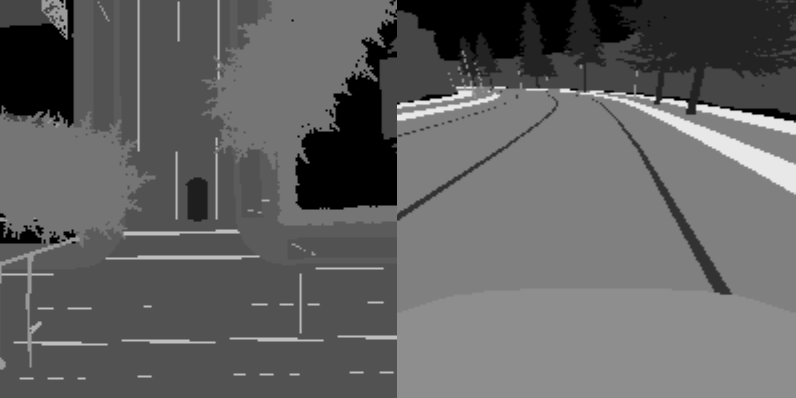
\includegraphics[scale=.271]{gt_combined.png}
    }}
    \caption{left: Ground truth segmented bird's eye view image, 64x64 in grayscale, 9 classes
    right: Ground truth segmented front view image, 80x80 in grayscale, 9 classes}
        \label{figurelabel}
        \end{figure}

\paragraph{Ground truth segmented frontview}
Much like the Ground truth segmented bird's eye view, the corresponding front view input representation assumes the availability of a 
perfect segmentation camera. Nonetheless, we increase realism with this representation as the camera is placed in front of the car.
Again, we chose a 13-class, 1-channel grayscale image with a slightly increased size of 80x80 to account for a larger view angle of the 
camera. 
\paragraph{Latent space generated from ground truth segmented images}
In this section we will further discuss a modified version of the integrated encoder-decoder network that is based on 
dziubinski's \cite{dziubinskiSemanticSegmentationSemantic2019} implementation. 
The underlying idea of this model is to 
guide feature extraction towards more useful, problem-specific features by exposing the model to the additional 
target of reconstructing a bird's eye view from the vehicle-based camera images.
In its original architecture, the network comprises 
5 input tensors and 7 output tensors with the inputs representing images of a front-, rear-, left-, right, and top-view camera. The 
model is built with the Keras functional API and generally serves two purposes. On the one hand, each input tensor is encoded into 
a 64-sized feature vector and decoded into it's original shape with a cross entropy loss with regard to the original input. This is 
achieved with separate branches of autoencoders with 3 convolutions respectively. On the other 
hand, a separate generative branch creates a bird's eye view reconstruction based on the concatenated feature vectors of the 
vehicle-based cameras. In addition to the cross entropy loss at the reconstructed bird's eye view output, a mean square error 
loss is calculated against the output of a subtract layer between the autoencoder's feature vector und the reconstructed feature vector to support
convergence. Notably, the autoencoder branch of the top-down camera view is solely purposed for improving the latent space of the generative branch 
during training and is thus not required for inference. 
\newline In comparison to dziubinski's \cite{dziubinskiSemanticSegmentationSemantic2019} vanilla version, we 
adjusted the architecture to fit the single camera bottlenecks into a length 64 vector and the reconstructed bird's eye view
bottleneck into a length 128 vector. To reduce complexity, we condensed both input and target segmentation images to 3 classes 
and implemented a generalized weighted cross entropy\cite{zhangGeneralizedCrossEntropy2018} loss function to 
account for the unbalanced distribution of vehicles and obstacles.
\begin{figure}[thpb]
   \centering
   \framebox{\parbox{3in}{
   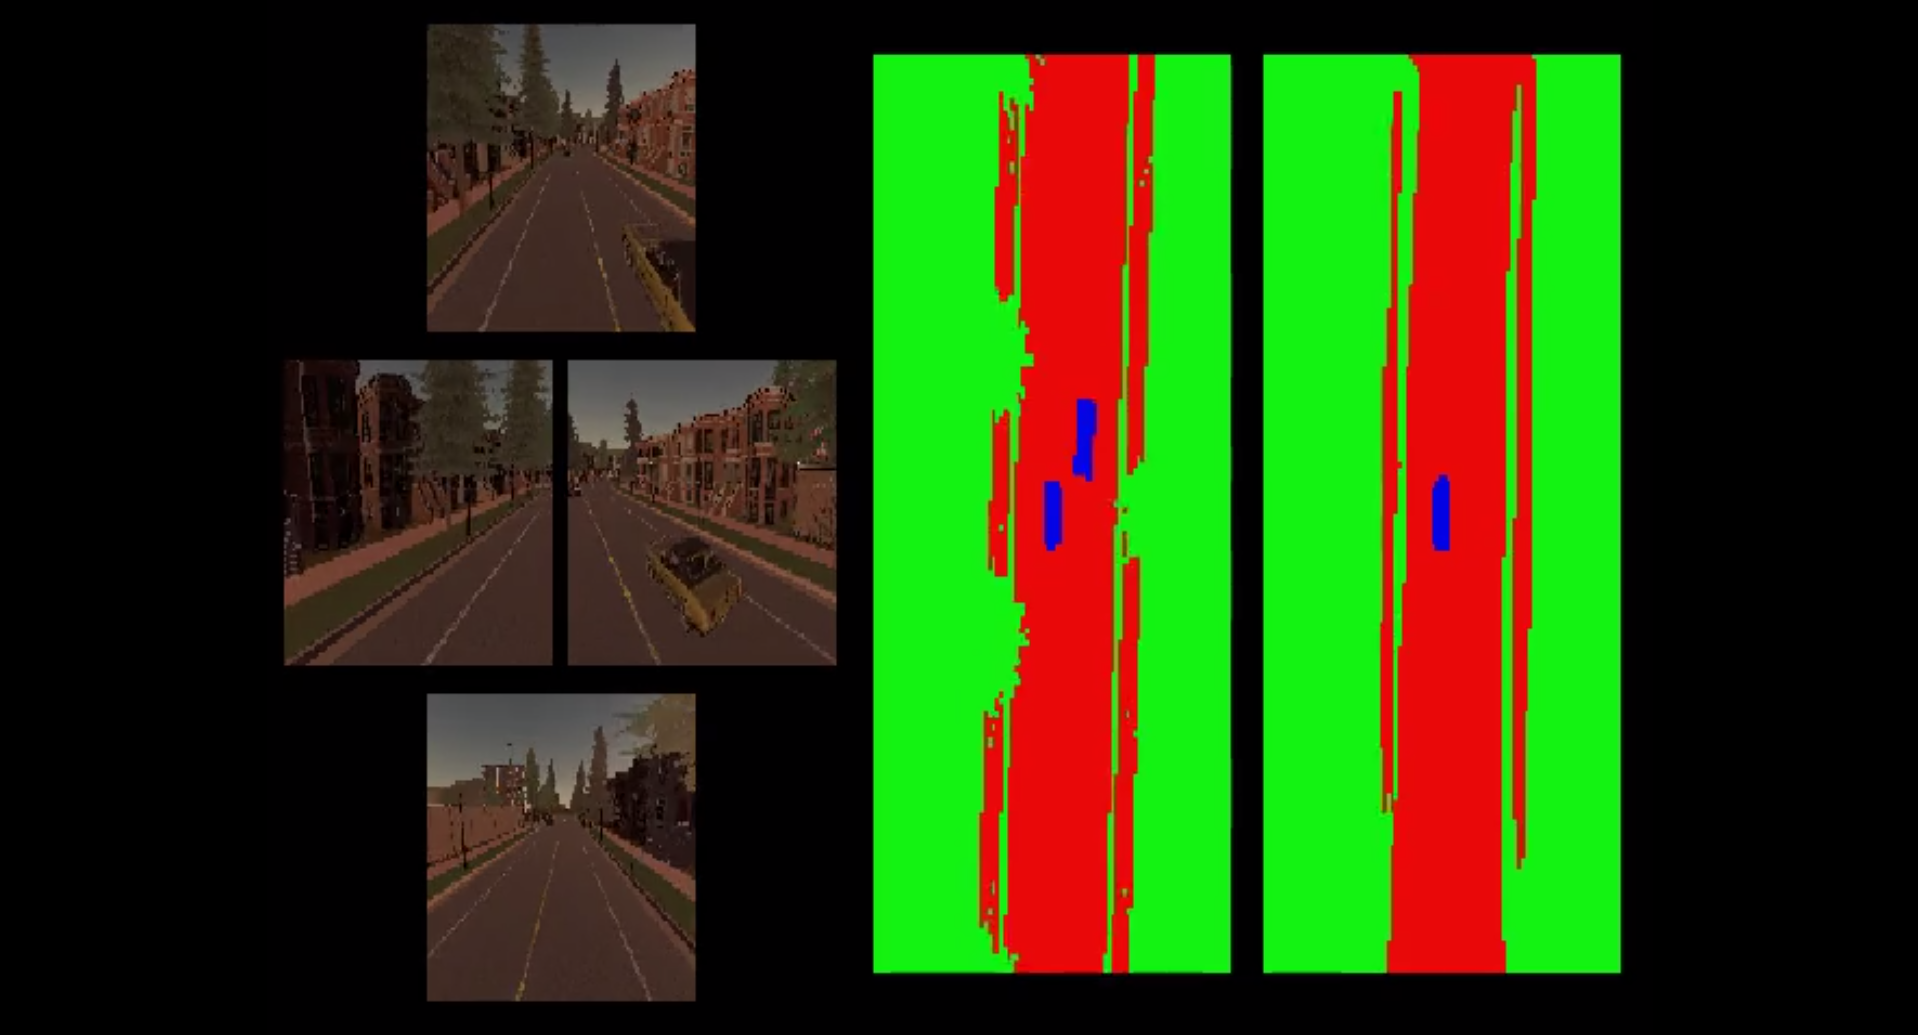
\includegraphics[scale=.113]{rgb_birdseye.png}
   }}
   \caption{left: rgb images from 4 vehicle-based cameras
            \newline 2nd from right: ground truth segmented bird's eye view
            \newline right: reconstructed bird's eye view}
       \label{figurelabel} 
       \end{figure}

\paragraph{Latent space generated from rgb images} To deal with the higher input complexity in RGB-images, we extended the
encoder and decoder models to 5 convolutions.
       
\subsection{Autoencoder/Latent space}
TODO: Encoder-decoder architecture bzw. Generator nennen
\subsection{Training}
In order to align the algorithms with the varying input dimensions we had to implement a wrapper around the actual models that adjusts the network architecture accordingly. Especially the fact that the latent space is flattened and not 2-dimensional such as the ground truth pictures made it neccessary to implement convolutional as well as  fully connected networks. Luckily, for the stable-baselines PPO model this is implemented very quickly. The architecture of our Keras-DDPG model however, had to be adjusted completely. 
We performed the training in four process steps, aligned with the input representation types mentioned previously. Therefore, the initial training was carried out on the ground-truth front view, afterwards on the ground-truth bird's eye view and finally we trained on the latent space of rgb and ground-truth segmented images. 
\subsubsection{DDPG}
The Deep Deterministic Policy Gradient performed well on our initial attempts within gym CarRacing and we identified reasonable hyperparameters for proper learning. We applied the same model on the new input features of CARLA and came to the sobering result that the input seemed to be too complex for the model. We assume, that the learning algorithm was distracted by the advanced simulation environment. The following illustration emphasizes the poor behavior of the model (trained on circumstances where other models performed well). Hence, we decided to continue with different learning approaches and agreed due to recent developments on the PPO.
\begin{figure}[thpb]
	\centering
	\framebox{\parbox{3in}{
			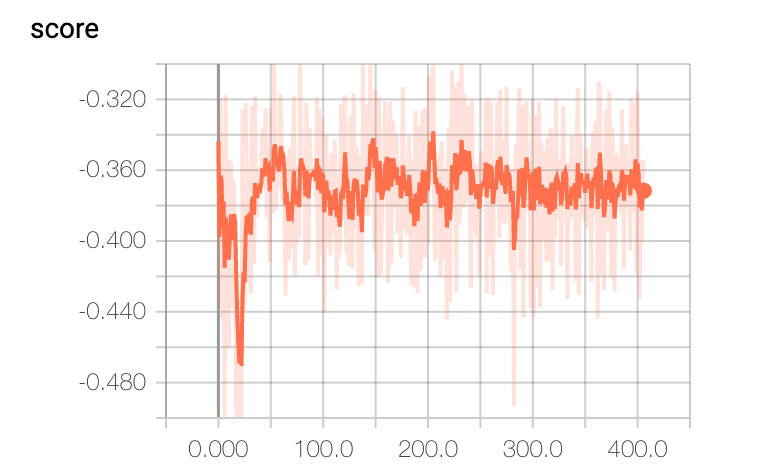
\includegraphics[scale=.5]{ddpg.png}
	}}
	\caption{Keras DDPG learning behavior}
	\label{figurelabel}
\end{figure}

\subsubsection{PPO}
The stable-baselines PPO2 model is easy to train and only few hyperparameters need to be adjusted. The drawback of this approach is that customization of these pre-defined models is rather laborious. Especially a combination of diverse input types such as scalars and images requires arduos architecture adjustments. We changed the following parameters and arrived at a very fast and crisp learning behavior that enables the agent to start driving after already very few episodes.

\begin{table}[!h]
	\footnotesize
	\centering
	\caption{Final reward function terms and weights}%
	\label{tab:Example}%
	\begin{tabularx}{\linewidth}{lcX}%
		\toprule
		\textbf{Parameter} & \textbf{Default Value} & \textbf{Selected Value} \\
		\midrule
		\makecell[Xt]{Learning rate}   & \makecell[Xt]{0.00025}  &\makecell[lt]{0.0004} \\
		\makecell[Xt]{Clip range}   & \makecell[Xt]{0.2}  &\makecell[lt]{0.1} \\
		\makecell[Xt]{Gamma}   & \makecell[Xt]{0.99}  &\makecell[lt]{0.97} \\
		\makecell[Xt]{N\_steps}   & \makecell[Xt]{128}  &\makecell[lt]{1024} \\
		\makecell[Xt]{Environment steps}   & \makecell[Xt]{25k}  &\makecell[lt]{200k} \\
	\end{tabularx}
\end{table}

The learning behavior usually increased until 200k steps and started to stagnate afterwards. The achieved episode rewards and entropy loss over several runs was very stable and performance drops occured rarely. The results on the proved input representations were very different: We trained the PPO with the same reward function, the same amount of steps at the same environment spawn point and hence assumed equal conditions. The front-cam-view resulted in a very oscilating driving behavior and the rewards were damped by the penalties for inaccurate delta heading. The birds-eye-view on the other hand had a very smooth driving behavior and deliverd the best performance in our test. This comes from the improved view on the street trajectory from above. Considering the easier and smaller latent space representation we realized that the algorithm trains very fast but can't reproduce the performance of the ground-truth. We assume that the architecture didn't contain the complete information in the layers that were extracted in our experiment and hence the latent space should usually arrive at a similar outcome as the ground-truth birds-eye-view.


\begin{figure}[thpb]
	\centering
	\framebox{\parbox{3in}{
			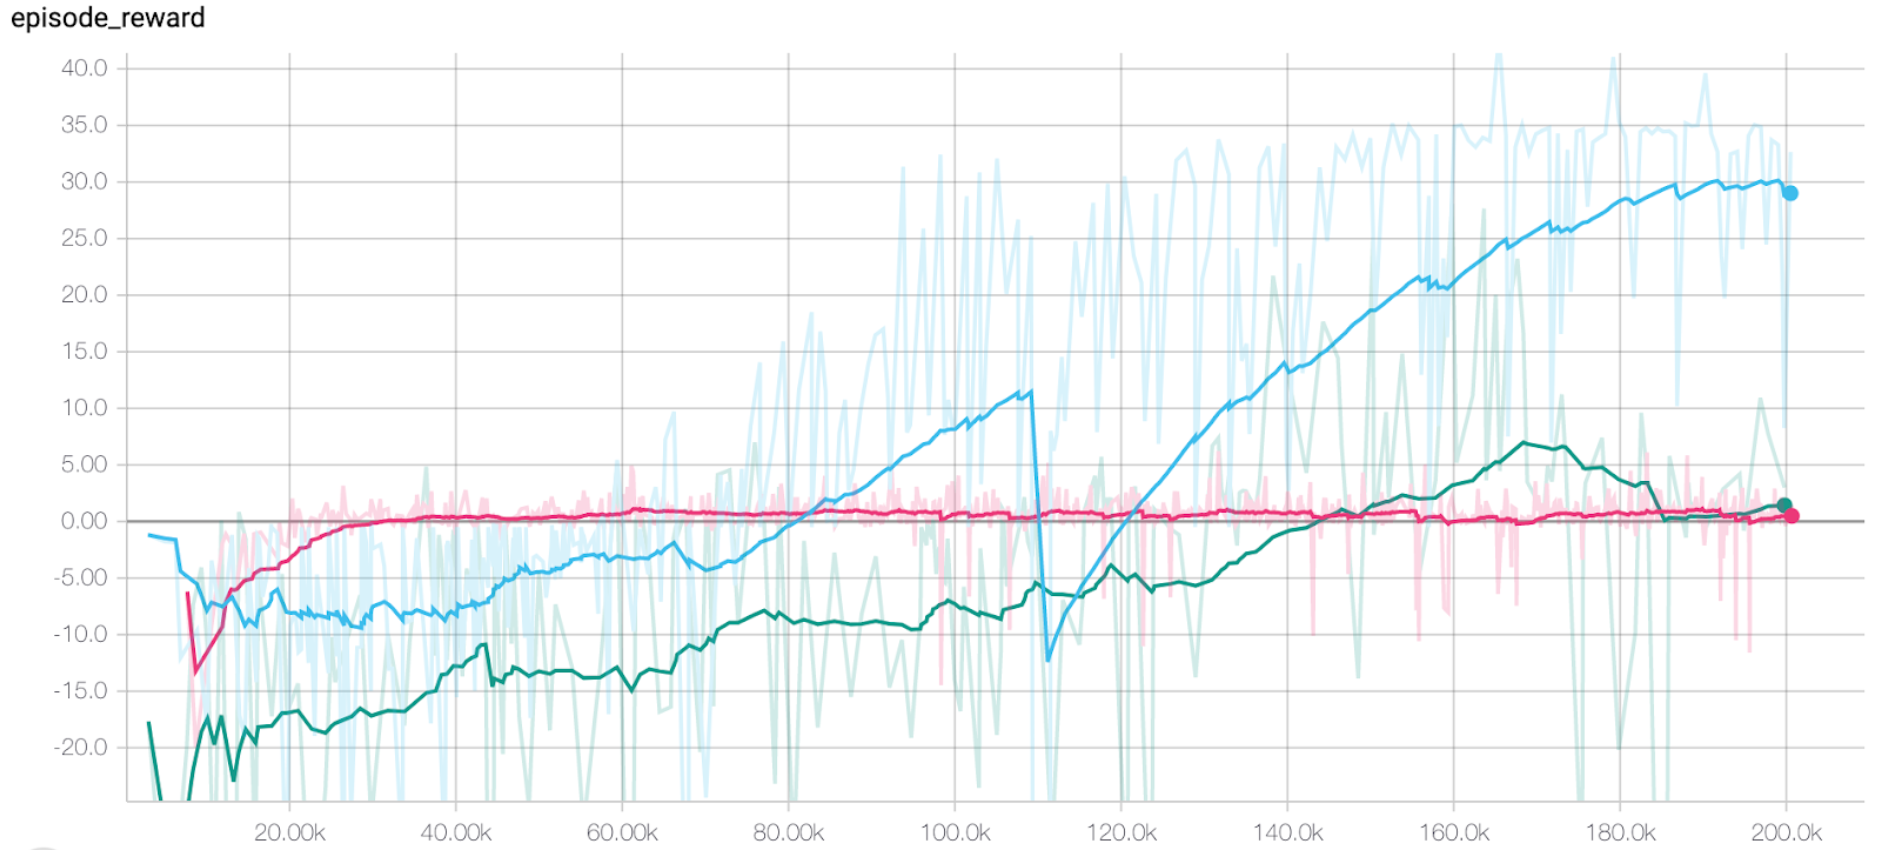
\includegraphics[scale=.23]{comparison_rewards.png}
	}}
	\caption{Green line: Performance on front-cam-view, Blue line: Performance on birds-eye-view, Red line: Performance on latent space}
	\label{figurelabel}
\end{figure}


%\subsection{CARLA}

\section{Evaluation}
\subsection{CarRacing-v0}
Due to the simple input structure and the straight-forward reward system we achieved stable results, even with using not the most-advanced learning algorithms (We consider the PPO as an improvement over the DDPG). Also the A3C could generate promising results (average rewards around 700) with only few training time.  In total, these results can be explained by the simplicity of the environment. However, here we invested more time on the finetuning of the hyperparameters compared with CARLA.
\subsection{CARLA}
The CARLA simulation environment is far more complex than the previous environment we worked with. Additionally, it was neccessary to implement the observations, terminal conditions as well as the reward function, where a lot of time was invested. The application of the stable-baselines algorithms is rather straight-forward. Hence, the challenging part here was merely the environment itself. 
\subsection{Results}
TODO: Mit Concept vergleichen und formulieren welche Ziele erreicht wurden / wo es probleme gab (analog zur präsi)

--- mo
Despite the weighted categorical cross entropy loss, the network struggled with
reconstructing pixels of the \textit{vehicle and obstacles} class. 
Aside from improving training data and network parameters, we 
consider a more sophisticated encoding model as crucial for better results. 
--- mo
\subsection{Comparison algorithms/reward functions}

\section{Conclusions}
As result of this practical seminar we have successfully applied different deep reinforcement approaches to the CARLA environment and finally achieved a stable and promising lane-keeping behavior for the agent. This was achieved by a combination of finding the most suitable input representation for smooth driving, finetuning of the rewardfunction and identification of the best performing hyperparameters. The outcome proves that reinforcement learning can be applied to complex environments as well as long as the desired behavior is incooperated in the reward system. Furthermore, we could prove that the birds-eye-view leads to a better performance as a single front camera and is also feasible in a real-world setup by generating the representation from four cameras surrounding the car. In the training process we recommend to not use early-termination for the episodes, especially if the reward function contains negative components, since this increases the probability that the agent starts to drive off the track as soon as possible. Finally, we emphasize that the driving behavior has the potential to be even further improved in the future by selecting better data, learning algorithms and an optimal reward function. We can also imagine, that the involvement of further attributes in the model such as the current velocity can be used to describe even more complex driving situations.  \newline
For the future we additionally suggest a combination of the birds-eye-view with a front camera in order to enable the identification of traffic signs and traffic lights, which wouldn't be possible from above. Also, we assume that the improvement of the encoder-decoder architecture could boost the learning speed and overall performance.




\begin{itemize}
      \item Similar to the abstract but more detail
      \item Conclusion of the key points of each section
      \item Summary of main findings
      \item Important conclusions that can be drawn
      \item Discuss benefits and shortcomings of our approach
      \item Suggest future areas of research
   \end{itemize}


\addtolength{\textheight}{-12cm}   % This command serves to balance the column lengths
                                  % on the last page of the document manually. It shortens
                                  % the textheight of the last page by a suitable amount.
                                  % This command does not take effect until the next page
                                  % so it should come on the page before the last. Make
                                  % sure that you do not shorten the textheight too much.

%%%%%%%%%%%%%%%%%%%%%%%%%%%%%%%%%%%%%%%%%%%%%%%%%%%%%%%%%%%%%%%%%%%%%%%%%%%%%%%%



%%%%%%%%%%%%%%%%%%%%%%%%%%%%%%%%%%%%%%%%%%%%%%%%%%%%%%%%%%%%%%%%%%%%%%%%%%%%%%%%



%%%%%%%%%%%%%%%%%%%%%%%%%%%%%%%%%%%%%%%%%%%%%%%%%%%%%%%%%%%%%%%%%%%%%%%%%%%%%%%%

%References are important to the reader; therefore, each citation must be complete and correct. If at all possible, references should be commonly available publications.










\newpage

\bibliographystyle{IEEEtran}
\bibliography{IEEEabrv,04_mendeley-export/library}


\newpage

\appendices



\end{document}
